\section{Auswertung}
\label{sec:Auswertung}

% % Examples
% \begin{equation}
%   U(t) = a \sin(b t + c) + d
% \end{equation}
%
% \begin{align}
%   a &= \input{build/a.tex} \\
%   b &= \input{build/b.tex} \\
%   c &= \input{build/c.tex} \\
%   d &= \input{build/d.tex} .
% \end{align}
% Die Messdaten und das Ergebnis des Fits sind in Abbildung~\ref{fig:plot} geplottet.
%
% %Tabelle mit Messdaten
% \begin{table}
%   \centering
%   \caption{Messdaten.}
%   \label{tab:data}
%   \sisetup{parse-numbers=false}
%   \begin{tabular}{
% % format 1.3 bedeutet eine Stelle vorm Komma, 3 danach
%     S[table-format=1.3]
%     S[table-format=-1.2]
%     @{${}\pm{}$}
%     S[table-format=1.2]
%     @{\hspace*{3em}\hspace*{\tabcolsep}}
%     S[table-format=1.3]
%     S[table-format=-1.2]
%     @{${}\pm{}$}
%     S[table-format=1.2]
%   }
%     \toprule
%     {$t \:/\: \si{\milli\second}$} & \multicolumn{2}{c}{$U \:/\: \si{\kilo\volt}$\hspace*{3em}} &
%     {$t \:/\: \si{\milli\second}$} & \multicolumn{2}{c}{$U \:/\: \si{\kilo\volt}$} \\
%     \midrule
%     \input{build/table.tex}
%     \bottomrule
%   \end{tabular}
% \end{table}
%
% % Standard Plot
% \begin{figure}
%   \centering
%   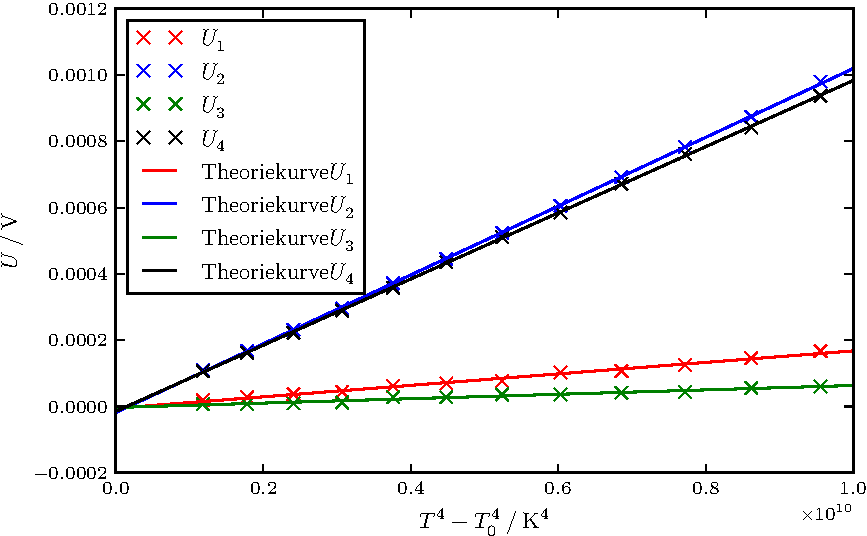
\includegraphics{build/plot.pdf}
%   \caption{Messdaten und Fitergebnis.}
%   \label{fig:plot}
% \end{figure}
%
% 2x2 Plot
% \begin{figure*}
%     \centering
%     \begin{subfigure}[b]{0.475\textwidth}
%         \centering
%         \includegraphics[width=\textwidth]{Abbildungen/Schaltung1.pdf}
%         \caption[]%
%         {{\small Schaltung 1.}}
%         \label{fig:Schaltung1}
%     \end{subfigure}
%     \hfill
%     \begin{subfigure}[b]{0.475\textwidth}
%         \centering
%         \includegraphics[width=\textwidth]{Abbildungen/Schaltung2.pdf}
%         \caption[]%
%         {{\small Schaltung 2.}}
%         \label{fig:Schaltung2}
%     \end{subfigure}
%     \vskip\baselineskip
%     \begin{subfigure}[b]{0.475\textwidth}
%         \centering
%         \includegraphics[width=\textwidth]{Abbildungen/Schaltung4.pdf}    % Zahlen vertauscht ... -.-
%         \caption[]%
%         {{\small Schaltung 3.}}
%         \label{fig:Schaltung3}
%     \end{subfigure}
%     \quad
%     \begin{subfigure}[b]{0.475\textwidth}
%         \centering
%         \includegraphics[width=\textwidth]{Abbildungen/Schaltung3.pdf}
%         \caption[]%
%         {{\small Schaltung 4.}}
%         \label{fig:Schaltung4}
%     \end{subfigure}
%     \caption[]
%     {Ersatzschaltbilder der verschiedenen Teilaufgaben.}
%     \label{fig:Schaltungen}
% \end{figure*}

\subsection{\texorpdfstring{Bestimmung der Reichweite und des Energieverlustes von $\alpha$-Strahlung}{Bestimmung der Reichweite und des Energieverlustes von Alpha-Strahlung}.}

\subsubsection{\texorpdfstring{Auswertung für $s=\SI{2.5}{\centi\metre}$}{Auswertung für s = 2.5 cm}.}

Nach der in der Durchführung beschriebenen Vorbereitung wird die erste Messung bei einem Abstand von $s = \SI{2.5}{\centi\metre}$ durchgeführt, die Messintervalle betragen $\increment t = \SI{120}{\second}$.
Die Drücke werden im Abstand $\increment p = \SI{50}{\milli\bar}$ bzw. für Bereiche mit starken Änderungen der Zählrate im Abstand von $\increment p = \SI{25}{\milli\bar}$ variiert und nach Formel \eqref{eqn:xeff} in effektive Längen umgerechnet.
Diese Messwerte sind in Tabelle \ref{tabulatore} einzusehen.

\input{build/tabulatore.tex}

Das Ergebnis der Zählrate in Abhängigkeit der effektiven Länge ist in Abbildung \ref{abb:2}, das der mittleren Energie in Abhängigkeit der effektiven Länge in Abbildung \ref{abb:3} dargestellt.

\begin{figure}
  \centering
  \includegraphics{build/plot_a_1.pdf}
  \caption{Ergebnisse der Zählrate in Abhängigkeit der mittleren Reichweite für $s = \SI{2.5}{\centi\metre}$.}
  \label{abb:2}
\end{figure}

Zur graphischen Bestimmung der mittleren Reichweite der $\alpha$-Teilchen wird die maximale Zählrate zu $\num{46500}$ Impulsen abgelesen, die Hälfte der Zählrate zu $\num{23000}$ Impulsen.
Beide Werte sind als blaue horizontale Linien in der Abbildung angegeben.
Werden die Werte um die Kante nun linear gefittet, ergibt sich, dass sich die Zählrate bei einer effektiven Länge von
\begin{align*}
  x_\text{mit} &= \input{build/x_mittel_1.tex}
\end{align*}
halbiert hat.
Wird die Energieskala als linear angenommen mit einer maximalen Energie von $\SI{4}{\mega\electronvolt}$ bei dem höchsten Channel von $\num{1023}$, so entspricht $x_\text{mit}$ einem Channel von $\num{406}$ und somit einer Energie von
\begin{align*}
  E_\text{mit} &= \input{build/E_mittel_1.tex}.
\end{align*}

\begin{figure}
  \centering
  \includegraphics{build/plot_a_1_1.pdf}
  \caption{Ergebnisse der mittleren Energie in Abhängigkeit der mittleren Reichweite für $s = \SI{2.5}{\centi\metre}$.}
  \label{abb:3}
\end{figure}
Zur Bestimmung des Energieverlustes $-\frac{\symup{d}E}{\symup{d}x}$ wird eine lineare Regression für die mittlere Energie in Abhängigkeit der effektiven Weglänge durchgeführt.
Dabei werden die blau markierten Messwerte verwendet, welche sich für einen linearen Zusammenhang eignen.
Der Fit wird mit SciPy in Python durchgeführt und ergibt die Parameter
\begin{align*}
  m_1 &= \input{build/parameter_a_1.tex},\\
  b_1 &= \input{build/parameter_b_1.tex}.
\end{align*}
Hieraus lässt sich $m_1$ als Energieverlust indentifizieren.

\subsubsection{\texorpdfstring{Auswertung für $s=\SI{1.5}{\centi\metre}$}{Auswertung für s = 1.5 cm}.}
Die zuvor beschriebene Messreihe wird analog für den Abstand $s = \SI{1.5}{\centi\metre}$ durchgeführt.
Es ergeben sich für die Zählrate in Abhängigkeit der effektiven Länge die in Abbildung \ref{abb:4} dargestellten Messwerte, für die mittlere Energie in Abhängigkeit der effektiven Länge die in Abbildung \ref{abb:5} dargestellten Messwerte.

\begin{figure}
  \centering
  \includegraphics{build/plot_a_2.pdf}
  \caption{Ergebnisse der Zählrate in Abhängigkeit der mittleren Reichweite für $s = \SI{1.5}{\centi\metre}$.}
  \label{abb:4}
\end{figure}

Aufgrund des zu geringen Abstandes vom Detektor zur Quelle halbiert sich im Bereich der Messreihe die Anzahl der Impulse nicht, so dass die mittlere Reichweite aus dieser Messreihe nicht bestimmt werden kann.
Es kann lediglich die Aussage getroffen werden, dass die mittlere Reichweite größer als $x_\text{mit} = \SI{1.5}{\centi\metre}$ ist.

\begin{figure}
  \centering
  \includegraphics{build/plot_a_2_2.pdf}
  \caption{Ergebnisse der mittleren Energie in Abhängigkeit der mittleren Reichweite für $s = \SI{1.5}{\centi\metre}$.}
  \label{abb:5}
\end{figure}

Zur Berechnung des Energieverlustes werden die blau markierten Werte verwendet, welche auf einer Gerade liegen.
Der lineare Fit mit SciPy ergibt die Parameter
\begin{align*}
  m_2 &= \input{build/parameter_a_2.tex},\\
  b_2 &= \input{build/parameter_b_2.tex},
\end{align*}
hier bezeichnet $m_2$ ebenfalls den Energieverlust.

\subsection{Statistische Auswertung der Zählraten}
\subsubsection{Vergleich mit Gaußverteilung}
Für die statistische Auswertung werden für $\num{100}$ Messeinheiten die Zählraten im Zeitintervall $\increment t = \SI{10}{\second}$ gemessen.
Der Abstand vom Detektor zur Quelle beträgt $s = \SI{1.5}{\centi\metre}$.
Aus den Messwerten ergibt sich nach Formel \eqref{eq:std_mean} ein Mittelwert der Zählraten von
\begin{align*}
  \mu &= \input{build/mu_stat.tex}
\end{align*}
sowie eine Standardabweichung von
\begin{align*}
  \sigma &= \input{build/sigma_stat.tex}.
\end{align*}
Zunächst wird mit diesen Werten eine Gaußverteilung um die Messwerte gelegt.
Dazu wird die allgemeine Formel der Gaußverteilung
\begin{equation}
  p(x) = \frac{1}{\sigma \sqrt{2 \pi}} \exp{\Bigl(-\frac{1}{2} \bigl( \frac{x-\mu}{\sigma} \bigr)^2 \Bigr)}
\end{equation}
verwendet.
Zudem wird ein Histogramm mit $\num{10}$ Bereichen erstellt.
Das Ergebnis ist in Abbildung \ref{abb:6} dargestellt.

\begin{figure}
  \centering
  \includegraphics{build/plot_stat.pdf}
  \caption{Gaußverteilung zu den Zählraten.}
  \label{abb:6}
\end{figure}

\subsubsection{Vergleich mit Poissonverteilung}
Für die Poissonverteilung wird ebenfalls ein Histogramm mit $\num{10}$ Bereichen erstellt.
Die Poissonverteilung wird mithilfe von SciPy in Python erstellt.
Es ergibt sich die in Abbildung \ref{abb:7} dargestellte Darstellung.

\begin{figure}
  \centering
  \includegraphics{build/statistik.pdf}
  \caption{Poissonverteilung zu den Zählraten.}
  \label{abb:7}
\end{figure}
